\section{Methods}
\label{sec:method}

\subsection{Minutiae Graph}
To build minutiae graph, we need to determine vertex and edge for the graph. The most intuitive way to determine the vertex is by choosing the minutiae as the vertex. Here, each vertex is represented by the minutiae pixel location $(x, y)$ from the original fingerprint image. For the edge configuration, there are two ways to connect the vertices by edges. One way is to connect each vertex with its $k$ nearest neighbor and the number $k$ is preset by the user. However, this method is sensitive to missing or spurious minutiae. The other way is to connect the vertices through triangulation. We use Delaunay triangulation method to form the edges here.

% \begin{figure}[htb]
%     \begin{minipage}[b]{0.48\linewidth}
%         \centering
%         \centerline{\epsfig{figure=mnt_overlay.png, width=4.0cm}}
%         \caption{Minutiae}
%         \label{fig:mnt_over}
%     \end{minipage}
%     \hfill
%     \begin{minipage}[b]{0.48\linewidth}
%         \centering
%         \centerline{\epsfig{figure=triangulation.png, width=4.0cm}}
%         \caption{Triangulation}
%         \label{fig:triang}
%     \end{minipage}
% \end{figure}


% \begin{figure}[htb]
% \centering
% \subfigure[Minutiae]{\epsfig{figure=./image/fingerprint1_1/mnt_overlay.png, height=4.0cm}}
% \hspace{0in}
% \subfigure[Triangulation]{\epsfig{figure=./image/fingerprint1_1/triangulation.png, width=4.0cm, height=4.0cm}}
% \hspace{0in}
% \subfigure[Triangulation]{\epsfig{figure=./image/fingerprint1_1/mnt_graph.png, width=4.0cm, height=4.0cm}}
% \caption{Fingerprint1_1}
% \label{fig:fingerprint1_1}
% \end{figure}

    
\begin{figure*}[!ht]
    \centering
    \begin{minipage}[b]{0.93\linewidth}
        \subfloat[original fingerprint iamge and detected minutiae]{
            \begin{minipage}[b]{0.27\linewidth}
                \centering
                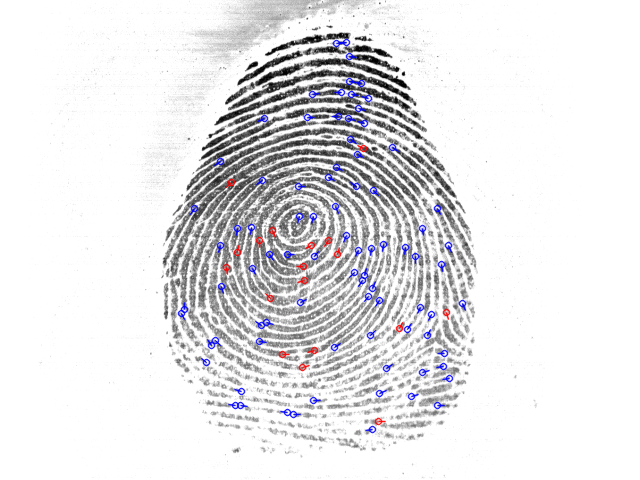
\includegraphics[height=4.0cm]{./image/fingerprint1_1/mnt_overlay.png}\vspace{8pt}
                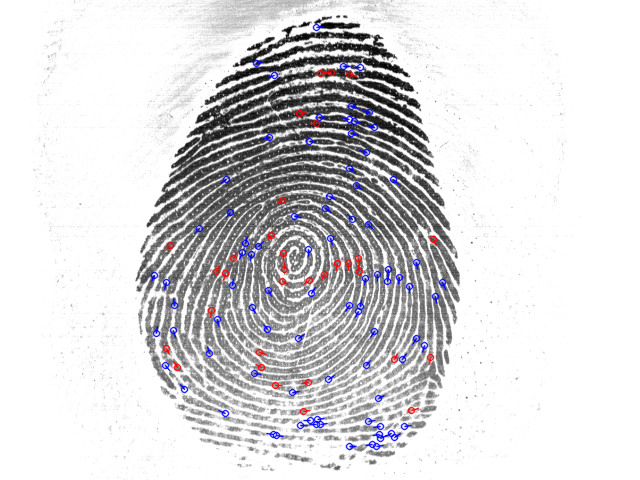
\includegraphics[height=4.0cm]{./image/fingerprint1_2/mnt_overlay.png}\vspace{8pt}
                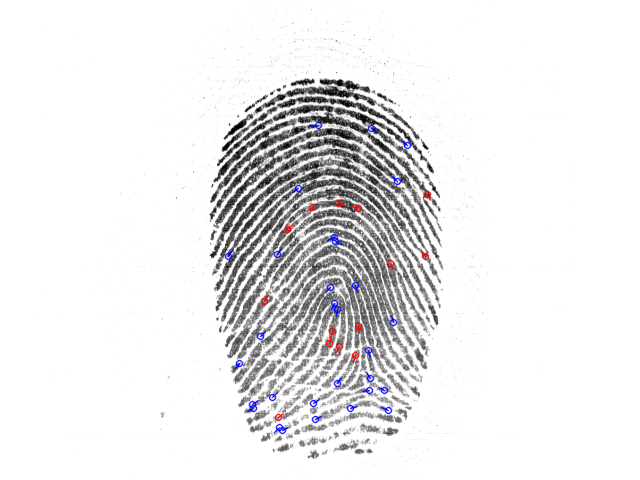
\includegraphics[height=4.0cm]{./image/fingerprint2_1/mnt_overlay.png}
            \end{minipage}
        }
        \hfill
        \subfloat[minutiae connected by triangulation]{
            \begin{minipage}[b]{0.27\linewidth}
                \centering
                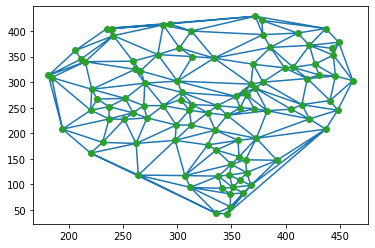
\includegraphics[width=\linewidth, height=4.0cm]{./image/fingerprint1_1/triangulation.png}\vspace{8pt}
                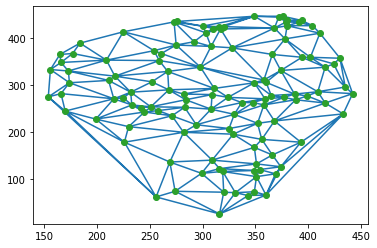
\includegraphics[width=\linewidth, height=4.0cm]{./image/fingerprint1_2/triangulation.png}\vspace{8pt}
                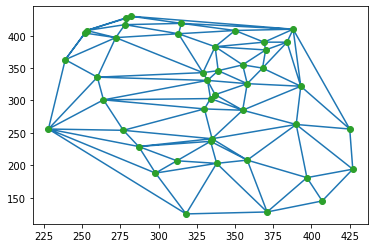
\includegraphics[width=\linewidth, height=4.0cm]{./image/fingerprint2_1/triangulation.png}
            \end{minipage}
        }
        \hfill
        \subfloat[minutiae graph visualization]{
            \begin{minipage}[b]{0.27\linewidth}
                \centering
                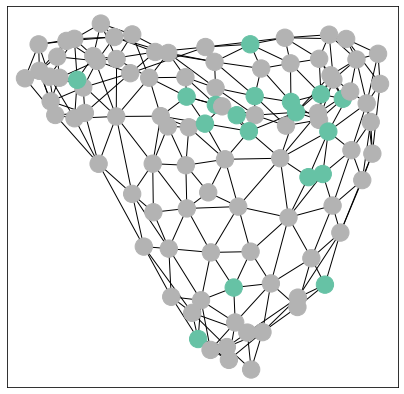
\includegraphics[width=\linewidth, height=4.0cm]{./image/fingerprint1_1/mnt_graph.png}\vspace{8pt}
                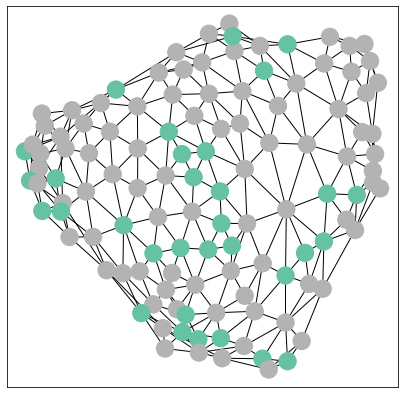
\includegraphics[width=\linewidth, height=4.0cm]{./image/fingerprint1_2/mnt_graph.png}\vspace{8pt}
                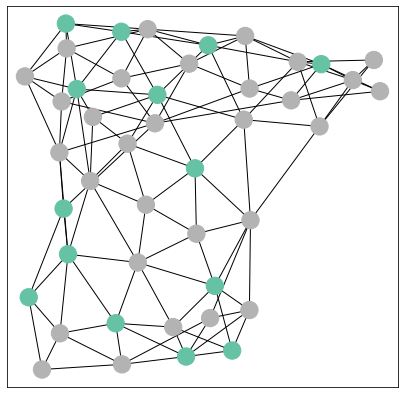
\includegraphics[width=\linewidth, height=4.0cm]{./image/fingerprint2_1/mnt_graph.png}
            \end{minipage}
        }
    \end{minipage}
    \vfill
    \caption{Sample fingerprint and its corresponding minutiae graph}
    \label{fig:mnt}
\end{figure*}

Figure \ref{fig:mnt} illustrates the way we build the minutiae graph. Each row shows one sample fingerprint image with detected minutiae and its corresponding minutiae graph. The left column shows the original fingerprint with detected minutiae that are plotted on it. The middle column shows the minutiae that are connected by Delaunay triangulation method. Note that because the origin of the fingerprint image is on the top left and the origin of the plot is on the bottom left, the minutiae that are plotted in the middle column are turned upside down compared with those minutiae in the left column. The right column shows the minutiae graph once the vertices and edges are built from the previous two columns. The geometric information of the minutiae is lost in the minutiae graph.